% Template adapted from https://github.com/sylvainschmitt/PhD/tree/master/documents/thesis/latex/template.latex

%%% STYLE %%%
\documentclass[12pt,twoside,a4paper, a]{article}



%%% PACKAGES %%%

% fonts
\usepackage{lmodern}
% \usepackage{anyfontsize}

\usepackage{lipsum}

% pdf
\usepackage{pdfpages}

% formulae
\usepackage{amssymb,amsmath}
\usepackage{ifxetex,ifluatex}
\usepackage{fixltx2e}
\usepackage[T1]{fontenc}
\usepackage[utf8]{inputenc}

% Tables
% pacakges for kableextra
\usepackage{booktabs}
\usepackage{longtable}
\usepackage{array}
\usepackage{multirow}
\usepackage{wrapfig}
\usepackage{float}
\usepackage{colortbl}
\usepackage{pdflscape}
\usepackage{tabu}
\usepackage{threeparttable}
\usepackage{threeparttablex}
\usepackage[normalem]{ulem}
\usepackage{makecell}
\usepackage{xcolor}
% \usepackage{longtable,booktabs}
% Fix footnotes in tables (requires footnote package)
\IfFileExists{footnote.sty}{\usepackage{footnote}\makesavenoteenv{long table}}{}

% graphics

% indent
\IfFileExists{parskip.sty}{%
\usepackage{parskip}
}{% else
\setlength{\parindent}{0pt}
\setlength{\parskip}{6pt plus 2pt minus 1pt}
}

% prevent overfull lines
\setlength{\emergencystretch}{3em}  
\providecommand{\tightlist}{%
\setlength{\itemsep}{0pt}\setlength{\parskip}{0pt}}

\setcounter{secnumdepth}{0}

% set default figure placement to htbp
\makeatletter 
\def\fps@figure{htbp}
\makeatother

% set default table placement to htbp
\makeatletter 
\def\fps@table{htbp}
\makeatother

% code highlights

% background image added by V.V.
\usepackage{eso-pic}
\newcommand\BackgroundIm{
\put(0,0){
  \parbox[b][\paperheight]{\paperwidth}{%
    \vfill
    \centering
    
\includegraphics[height=\paperheight,width=\paperwidth]{img/background.jpg}%
    \vfill
}}}

% packages added by V.V.
\usepackage{lettrine}
\usepackage{caption}

% For Pandoc 2.11+, added by V.V. from thesisdown
\newlength{\cslhangindent}
\setlength{\cslhangindent}{1.5em}
\newenvironment{CSLReferences}[2] % #1 hanging-ident, #2 entry spacing
 {% don't indent paragraphs
  \setlength{\parindent}{0pt}
  % turn on hanging indent if param 1 is 1
  \ifodd #1 \everypar{\setlength{\hangindent}{\cslhangindent}}\ignorespaces\fi
  % set entry spacing
  \ifnum #2 > 0
  \setlength{\parskip}{#2\baselineskip}
  \fi
 }%
 {}
 
% To pass between YAML and LaTeX, added by V.V. from thesisdown
\def\title#1{\def\title{#1}}
\title{TITRE SUFFISAMMENT COMPLIQUÉ POUR REFLÉTER LA GRANDE COMPLEXITÉ DU TRAVAIL}
\def\author#1{\def\author{#1}}
\author{Aubin SAHALOR}
\def\date#1{\def\date{#1}}
\date{01 Janvier 2001}
\def\supervisor#1{\def\supervisor{#1}}
\supervisor{Thérèse PONSABLE}
\def\specialty#1{\def\specialty{#1}}
\specialty{Écologie fonctionnelle et Sciences Agronomiques}
\def\department#1{\def\department{#1}}
\department{UMR 5175 -- Centre d'Ecologie Fonctionnelle et Evolutive - CNRS}

% paragraphs
% beware this make the toc bug if hyperref is placed before
\usepackage{titlesec}
\let\oldsection\section
\renewcommand\section{\clearpage\oldsection}
\titleformat{\section}
{\huge\center\scshape}{\thesection}{1em}{}[{\titlerule[0.5pt]}]
\titleformat*{\subsection}{\LARGE\bfseries}
\titleformat*{\subsubsection}{\Large\bfseries}
\titleformat*{\paragraph}{\large\bfseries\itshape}
\titleformat*{\subparagraph}{\normalsize\itshape}

% hyperlinks (cleverref and colors for UM added by V.V.)
\IfFileExists{upquote.sty}{\usepackage{upquote}}{}
\IfFileExists{microtype.sty}{%
\usepackage[]{microtype}
\UseMicrotypeSet[protrusion]{basicmath} % disable protrusion for tt fonts
}{}
\PassOptionsToPackage{hyphens}{url} % url is loaded by hyperref
\usepackage[unicode=true]{hyperref}
  \PassOptionsToPackage{usenames,dvipsnames}{color} % color is loaded by hyperref
\definecolor{um-red}{RGB}{233,78,82}
\definecolor{um-gray}{RGB}{114,146,162}
\hypersetup{
      colorlinks=true,
    linkcolor=um-red,
    citecolor=um-red,
    urlcolor=um-gray,
      breaklinks=true}
\urlstyle{same} % don't use monospace font for urls
\usepackage[capitalise, nameinlink]{cleveref}

% empty all blank pages created by \cleardoublepage, added by V.V.
\usepackage{emptypage}

% geometry
\usepackage[left=2.5cm,right=2.5cm,top=2cm,bottom=2cm]{geometry}
\renewcommand{\baselinestretch}{1.1}

% Bibliography
\usepackage{natbib}
\bibliographystyle{plainnat}

% citations
\usepackage{epigraph}

%%% BODY %%%
\begin{document}

% First pages
  \begin{titlepage}
    \newpage
    
    \AddToShipoutPicture*{\BackgroundIm}

    \let\footnotesize\small
    \let\footnoterule\relax
    \let \footnote \thanks

    \baselineskip = 1.4\baselineskip

    \begin{center}
    \setcounter{page}{1}
    
    \textbf{\textcolor{um-red}{\large{THÈSE POUR OBTENIR LE GRADE DE DOCTEUR} \\
    \large{DE L'UNIVERSITÉ DE MONTPELLIER} \\ }}
    
    \vspace*{\baselineskip} 
    \normalsize{\textbf{En \specialty}} \\
    \vspace*{\medskipamount} 
    \normalsize{\textbf{Ecole doctorale GAIA}} \\
    \vspace*{\medskipamount}
    \normalsize{\textbf{\department}} \\
    \vspace*{2cm}
    
    \textcolor{um-gray}{\Large{\textbf{\title}} \\ }
    \vspace*{1cm}
    
    \normalsize{\textbf{Présentée par \author}} \\
    \normalsize{\textbf{Le \date}} \\
    \vspace*{\baselineskip}
    
    \normalsize{\textbf{Sous la direction de \supervisor}} \\
    \vspace*{\fill}
    
    \normalsize{Devant le jury composé de} \\
    \begin{table}[h]
      \centering
      \makebox[0.9\columnwidth]{%
        \begin{tabular}{lllr}
          Prénom NOM             & Titre              & Affiliation                    & \emph{Rôle jury} \\
          Prénom NOM             & Titre              & Affiliation                    & \emph{Rôle jury} \\
          Prénom NOM             & Titre              & Affiliation                    & \emph{Rôle jury} \\
          Prénom NOM             & Titre              & Affiliation                    & \emph{Rôle jury} \\
          Prénom NOM             & Titre              & Affiliation                    & \emph{Rôle jury} \\
          Prénom NOM             & Titre              & Affiliation                    & \emph{Rôle jury} \\
          Prénom NOM             & Titre              & Affiliation                    & \emph{Rôle jury} \\
        \end{tabular}
      }
    \end{table}
    \end{center}
    
    \vspace*{\fill}
    
    \begin{center}
    
\includegraphics[width=0.4\columnwidth]{img/logo-um.png}
    \end{center}
    
  \end{titlepage}
  \newpage
  \null\vfill
  {\fontsize{7.5}{8}\selectfont
  \begin{center}
  \textbf{Titre en français} \\
  \end{center} 
  \textbf{Résumé :}
  \lipsum[1-4] \\

  \textbf{Mots clefs :}
  Motclef1; Motclef2; Motclef3 \vspace*{\baselineskip}
  \newline\noindent\rule{\textwidth}{0.7pt}

  \begin{center}
  \textbf{Title in English} \\
  \end{center} 
  \textbf{Abstract:}
  \lipsum[1-4]

  \textbf{Keywords:}
  Keyword1; Keyword2; Keyword3

  }
  \vfill\null
% 
% \tableofcontents
% \listoftables
% \listoffigures

\newpage

\pagenumbering{arabic}

\hypertarget{remerciements}{%
\section{Remerciements}\label{remerciements}}

\lipsum[1-6]

\setcounter{tocdepth}{2}
\tableofcontents
\listoftables
\listoffigures

\hypertarget{ruxe9sumuxe9-substantiel}{%
\section{Résumé substantiel}\label{ruxe9sumuxe9-substantiel}}

\hypertarget{introduction}{%
\subsection{Introduction}\label{introduction}}

\hypertarget{sous-titre}{%
\subsubsection{Sous-titre}\label{sous-titre}}

\lipsum[1-4]

\hypertarget{sous-titre-1}{%
\subsubsection{Sous-titre}\label{sous-titre-1}}

Just a paper with Pokemon related jokes which has strong implications for real-world species distribution modelling (\protect\hyperlink{ref-Warren2021}{Warren et al. 2021}).

\lipsum[5-6]

\hypertarget{chapitre-1-titre}{%
\subsection{Chapitre 1 : Titre}\label{chapitre-1-titre}}

\lipsum[7-9]

\hypertarget{chapitre-2-titre}{%
\subsection{Chapitre 2 : Titre}\label{chapitre-2-titre}}

\lipsum[10-11]

\hypertarget{etc.}{%
\subsection{Etc.}\label{etc.}}

\hypertarget{discussion}{%
\subsection{Discussion}\label{discussion}}

\lipsum[12-14]

\hypertarget{introduction-1}{%
\section{Introduction}\label{introduction-1}}

\hypertarget{title1}{%
\subsection{Title1}\label{title1}}

\hypertarget{subtitle}{%
\subsubsection{Subtitle}\label{subtitle}}

\lipsum[1]

\hypertarget{subtitle-1}{%
\subsubsection{Subtitle}\label{subtitle-1}}

\lipsum[2-3]

\hypertarget{subtitle-2}{%
\subsubsection{Subtitle}\label{subtitle-2}}

\lipsum[4-6]

\hypertarget{title2}{%
\subsection{Title2}\label{title2}}

\hypertarget{subtitle-3}{%
\subsubsection{Subtitle}\label{subtitle-3}}

\lipsum[1-3]

\begin{figure}[H]

{\centering 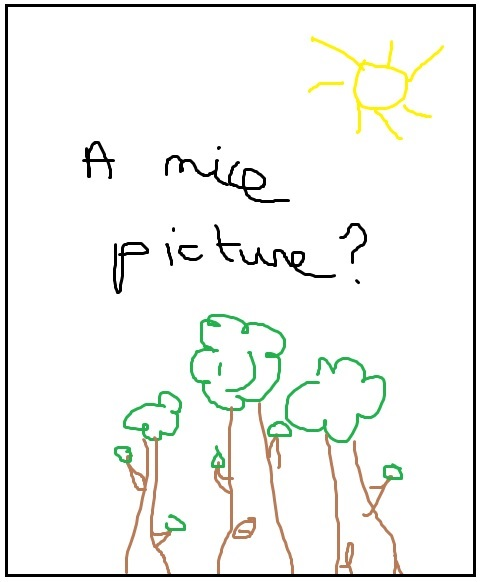
\includegraphics[width=\linewidth]{figures/nice_figure} 

}

\caption{What a nice drawing.}\label{fig:nicefigure}
\end{figure}

\hypertarget{subtitle-4}{%
\subsubsection{Subtitle}\label{subtitle-4}}

\lipsum[4-7]

\hypertarget{references}{%
\section*{References}\label{references}}
\addcontentsline{toc}{section}{References}

\hypertarget{refs}{}
\begin{CSLReferences}{1}{0}
\leavevmode\vadjust pre{\hypertarget{ref-Warren2021}{}}%
Warren, D. L. et al. 2021. The effects of climate change on australia's only endemic pokémon: Measuring bias in species distribution models. - Methods in Ecology and Evolution 12: 985--995.

\end{CSLReferences}

% \addcontentsline{toc}{section}{References}
\bibliography{bib/thesis.bib}
% \listoftables
% \listoffigures

% Last pages

\end{document}
